\documentclass[a4paper,12pt]{report}

\usepackage[serbian, ngerman, english]{babel}
\usepackage[a4paper, inner=3cm, outer=3cm, top=2cm, bottom=2cm]{geometry}
\usepackage{blindtext}
\usepackage{microtype}
\usepackage{graphicx}
\usepackage{wrapfig}
\usepackage{enumitem}
\usepackage{fancyhdr}
\usepackage{amsmath}
\usepackage{index}
\usepackage[autostyle]{csquotes}
\usepackage{amssymb}
%\usepackage{booktabs}

\makeindex
%after this beguins the document

\begin{document}
\selectlanguage{serbian} 
%\renewcommand{\contentsname}{Sadržaj}
%\renewcommand{\chaptername}{Poglavlje}

\title{\Large{\textbf{Logistička i softmaks regresija (opis metoda, implementacija, primena nad podacima, komparativna analiza) i njihova primena kao aktivacione funkcije u neuronskim mrežama }}}
\author{Student: Danilo Veljović, broj indeksa: 1120}
\date{Novembar 6, 2020}
\maketitle
\let\cleardoublepage\clearpage
\tableofcontents

\pagenumbering{arabic}

\setcounter{page}{1}

\chapter{Uvod}
\ Termini poput veštačke inteligencije i mašinskog učenja su sve popularniji u savremenoj kulturi. Preko medija sve češće čujemo nagoveštaje vodećih naučnika iz ove oblasti da će sistemi koji koriste veštačku inteligenciju zameniti ljude na mnogim radnim mestima. Priča se da će prvo nestati najrepetitivniji poslovi poput vozača kamiona, radnika u skladištima, prodavaca i dr. Treba postaviti suštinsko pitanje zašto je to tako. Zašto će prvo rutinski poslovi nestati prvi? Odgovor na to pitanje daje prave smernice kada neko pokušava da shvati šta je to mašinsko učenje. \\ 

Mašinsko učenje vuče korene iz statistike. Slobodno rečeno, mašinsko učenje se može shvatiti kao primena statističkih metoda nad velikom količinom podataka, da bi se izvukle nekakve pravilnosti iz podataka. Te pravilnosti uočava model i opisuje ih različitim statističkim terminima. Model se može shvatiti kao parametrizovana funkcija koja može da \enquote{uči} iz podataka. Podaci se u mašinskom učenju dele na trening i test skupove. Trening skupovi imaju određene vrednosti za atribute i imaju izlaznu labelu klase kojoj pripadaju ili neke kontinualne vrednosti koju uzimaju. Model uzima jedan po jedan podatak iz trening skupa, ili čitavu grupu, i proba da napravi predikciju koje bi izlazne vrednosti mogle da odgovaraju tim ulazima. Kada vidi koliko njegova procena odudara od vrednosti labele za taj podatak, on se ispravi svoje parametre. Ovaj proces se naziva treniranje modela. Kada model optimizuje svoje parametre, i kada se odradi evaluacija modela, prelazi se na testiranje. Kada se model testira njemu se daju instance podataka koje nikad nije video. Za te instance on sada predviđa izlazne labele. \\

Posle ovog kratkog objašnjenja procesa mašinskog učenja, lako se može naslutiti odgovor na prethodno postavljeno pitanje o poslovima koje će prvo 
\enquote{progutati} inteligentni sistemi. Uzmimo primer radnika koji radi u skladištu i pomera kutije od mesta A do mesta B. Robot može da posmatra radnika koji nosi kutije i da zaključi da radnik na mestu A podigne kutiju, nosi je do mesta B i tu je spušta. To je njegov \enquote{trening skup} podataka. Kod ovakvog tipa inteligentih sistema najčešće se koriste konvolucione neuronske mreže za računarski vid, pomoću kojih sistem prima podatke o tome šta se dešava oko njega. Princip ostaje isti, sistem preko kamera, prima ulazne podatke, i ovo služi kao trening skup podataka. Trenira određen model, i kada se završi taj proces on može da izvede zadatak prenosa kutija. Ako se od sistema zahteva da radi nešto novo, slično prethodnom, on će probati to da uradi na jedan način, i u zavisnosti od ishoda \enquote{učiće} o tome gde je pogrešio, odnosno optimizovaće model. \\

%sad malo o konkretnim tehnikama, logističkoj, softmaks regresiji i pregled rada nadalje
Tehnike mašinskog učenja su srž inteligentnih sistema. Neki od važnijih modela mašinskog učenja su: 
\begin{itemize}
	\item \textit{Klasifikacija} predviđa klasu koja odgovara podatku
	\item \textit{Regresija} predviđa kontinualnu vrednost koja odgovara podatku
	\item \textit{Klasterizacija} je tehnika nenadgledanog učenja. Za razliku od tehnika nadgledanog učenja, o kojima je do sad bilo reči, kod nenadgledanog učenja nemamo informaciju o tome koji podatak ima kakvu klasu/vrednost. Zadatak klasterizacije je da one podatke koji su \enquote{slični} (mera sličnost se definiše kao parametar tehnike) grupiše zajedno.
	\item \textit{Neuronske mreže} su tehnika koja je donela revoluciju u svet mašinskog učenja i omogućila stvari poput računarskog vida i procesuiranja prirodnih jezika. Ideja za ovu tehniku dobijena je iz ideje ljudskog mozga. Cela neuronska mreža se sastoji iz veštačkih neurona, koji su međusobno povezani. Na slici 1.1 dat je prikaz jedne neuronske mreže. Neuronska mreža se sastoji iz tri sloja, \textit{ulaznog} sloja, mnoštvo \textit{skrivenih} slojeva i \textit{izlaznog sloja}. Ideja kod funkcionisanja neuronske mreže je da početni slojevi prepoznaju jako male delove sistema, npr kod računarskog vida prepoznaju ivice, kod procesuiranja prirodnih jezika prepoznaju pojedina slova. Skriveni slojevi prepoznaju složenije pojave, npr geometrijske figure ili tela, ili reči i rečenice. Na kraju izlazni neuroni se aktiviraju ako je prepoznato nešto. Primera radi, mreža može da se trenira da prepoznaje slike mačaka ili da prepoznaje da li je neka rečenica nosi pozitivna ili negativna osećanja. Ako mreža prepozna sliku mačke, ili ako je određena rečenica ima pozitivna osećanja, izlazni neuron se aktivira. 
\end{itemize}

\begin{figure}[ht]
	\centering
	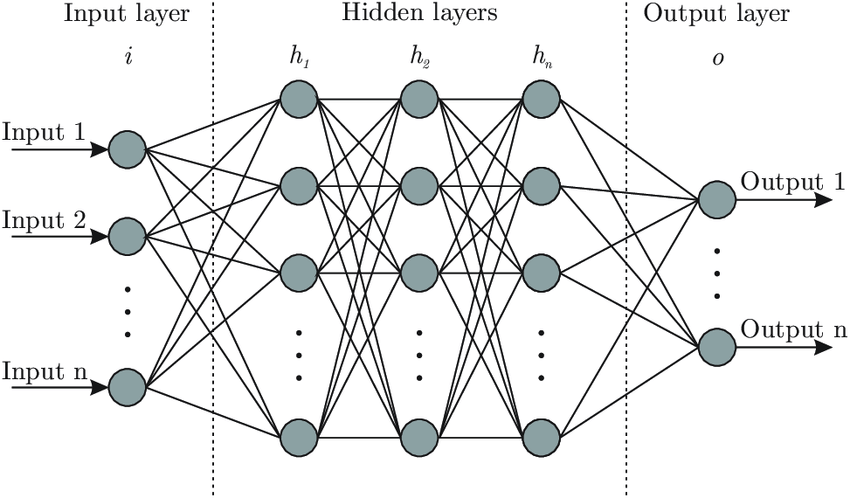
\includegraphics[width=8cm]{neuronske_mreze.png}
	\caption{Arhitektura neuronske mreže}\label{fig:prettypic}
\end{figure}

Jedna od tehnika koja se koristi za klasifikaciju se naziva \textit{logistička regresija}. Iako u nazivu sadrži reč \textit{regresija} ova tehnika se ne koristi za predviđanje kontinualne vrednosti, već za predviđanje da li neki podatak pripada nekoj klasi ili ne. U nastavku rada biće reči o matematičkim osnovama logističke regresije, o funkciji koja je vrlo slična logističkoj regresiji i vrlo često se koristi u sličnim situacijama - \textit{softmaks regresiji}. Implementiraćemo logističku i softmaks regresiju u programskom jeziku Python, primeniti je nad skupom podataka i evaluirati njihove performanse i napraviti komparativnu analizu obe tehnike. Na kraju rada biće dat prikaz primene logističke i softmaks regresije kao 
aktivacione funkcije (\enquote {\textit{threshold functions}}) kod neuronskih mreža.
\chapter{Teorijske osnove}

\section{Kratak pregled potrebnih pojmova iz verovatnoće i statistike}
Kako bi se pravilno razumela logistička regresija potrebno je pre toga dobro poznavati njene matematičke osnove. U nastavku je data kratka rekapitulacija potrebnih pojmova iz verovatnoće i statistike koji su potrebni za njeno razumevanje. Da bi se lakše svi pojmovi dati u nastavku, razmatrani su samo u okvirima diskretnih slučajnih promenljivih.\\

\subsection{Verovatnoća} 
Verovatnoća predstavlja odnos između broja ishoda u kome je neki događaj ispunjen i broja svih mogućih ishoda. 
\begin{equation} \label{eq:1}
	P = \frac{\textit{broj pozitivnih ishoda događaja}}{\textit{broj svih mogućih ishoda}} 
	%\caption{}
 \end{equation}
 
 \textit {Primer 1.} \
Primer jednog događaja može biti bacanje novčića. Pozitivan ishod je kada se padne glava. Broj svih mogućih ishoda u jednom bacanju je 2 (može se pasti ili pismo ili glava). Kada zamenimo ove vrednosti u prethodnu jednačinu dobijamo: 
\begin{equation} \label{eq:2}
	P = \frac{1}{2} = 0.5
	%\caption{}
 \end{equation}
Iz jednačine se vidi da je verovatnoća da u jednom bacanju novčića dobijemo glavu 0.5, odnosno 50 \%.

\subsection{Šansa}

Šansa predstavlja odnos između verovatnoće da se događaj desio i verovatnoće da se događaj nije desio.
\begin{equation} \label{eq:3}
	\textit{šansa} = \frac{\textit{P(događaj se desio)}}{\textit{P(događaj se nije desio)}} = \frac{\textit{p}}{\textit{1-p}}
	%\caption{}
 \end{equation}

Ako se vratimo na primer 1 bacanja novčića, vidimo da je šansa da se događaj desi, odnosno da se padne glava jednak: 
\begin{equation} \label{eq:4}
	\textit{šansa(glava)} = \frac{0.5}{0.5} = 1, tj. \textit{1:1}
	%\caption{}
 \end{equation}
 
 Zaključujemo da je šansa da se padne glava ista kao i šansa da se ne padne glava, tj 1 prema 1. 
 
 Odnos šansi se definiše kao:
 \begin{equation} \label{eq:4}
	\textit{odnos šansi} = \frac{\textit{šansa\textsubscript{1}}}{\textit{šansa\textsubscript{1}}} 
	%\caption{}
 \end{equation}
 
 \textit {Primer 2.} \ Uzmimo dva novčića, jedan koji je fer i drugi za koji se zna da je verovatnoća da se padne glava 0.7. Naći odnos šansi ova dva novčića za događaj kada se padne glava.\\
 Za fer novčić važi: 
 \begin{equation}
	P(glava) = \frac{1}{2} = 0.5 \\
	%\caption{}
 \end{equation}
 \begin{equation}
	\textit{šansa(glava)\textsubscript{fer}} = \frac{0.5}{0.5} = 1, tj. \textit{1:1}
	%\caption{}
 \end{equation}
 
 Za \enquote{nefer} novčić važi: 
  \begin{equation}
	P(glava) = 0.7
	%\caption{}
 \end{equation}
 \begin{equation}
	\textit{šansa(glava)\textsubscript{nefer}} = \frac{0.7}{0.3} = 2.333
	%\caption{}
 \end{equation}
 
 Odnos šansi definišemo kao: 
  \begin{equation}
	 \textit{odnos šansi} = \frac{\textit{šansa(glava)\textsubscript{nefer}}}{\textit{šansa(glava)\textsubscript{fer}}} = \frac{2.333}{1} = 2.333
 \end{equation}
 Vidi se da su šanse da se padne glava na \enquote(nefer) novčiću veća nego da se dobije glava na \enquote(fer) novčiću 2.333 puta. 
\subsection{Bernulijeva raspodela}

Bernulijevu raspodelu je najlakše razumeti kroz Bernulijev eksperiment. Bernulijev eksperiment je eksperiment koji se dešava jednom i koji kao rezultat može da ima uspeh (obično obeležen 1) ili neuspeh (obično obeležen 0) tj ima samo dve moguće posledice. Najbolji primer za to je bacanje novčića. Dve moguće posledice su da se padne ili pismo ili glava. Uzmimo da se uspešnim događajem smatra da se pala glava pri bacanju. Odavde sledi da ako se padne pismo, to smatramo neuspehom. Izvedemo eksperiment jednom i ako se padne glava smatramo da se desio uspešan događaj, ako se padne glava smatramo da se desio neuspešan događaj. \\

Definišemo slučajnu promenljivu $X$ = broj uspeha pri bacanju novčića i $X \sim Bernoulli(p)$. Moguće vrednosti koje slučajna promenljiva može da ima (obeležavamo ih sa x) su 0 ili 1. Nula se dobija ako se pri jednom bacanju nije desio uspešan događaj, odnosno 1 ako se desio uspešan događaj.  Obeležavamo to sa x = 0, 1. \\
Verovatnoća da se desio uspešan događaj je ujedno i jedini parametar distribucije, i obeležava se sa $p$.
  \begin{equation}
	 P(X = 1) = p 
 \end{equation}
Jedan parametar se prosleđuje jer imamo samo jedan eksperiment. Odavde se može primetiti da je Bernulijeva raspodela specijalan slučaj Binomne raspodele za $n = 1$.\\
Verovatnoća da se desio neuspešan događaj je:
\begin{equation}
	 P(X = 0) = 1-p = q 
 \end{equation}

Za primer fer bacanja novčića, verovatnoća uspeha je:
  \begin{equation}
	 P(X = 1) = 0.5 
 \end{equation}
Verovatnoća neuspeha je data u jednačini
  \begin{equation}
	 P(X = 0) = 0.5 
 \end{equation}
 
Očekivana vrednost (srednja vrednost) se za diskretne slučajne promenljive koje imaju Bernulijevu raspodelu dobija kao:  
   \begin{equation}
	 \mu = E[X] = \sum_{x\textsubscript{i} \in \mathcal{X}}^{\mathcal{X}} x\textsubscript{i} p(X = x\textsubscript{i}) = 1 * p + 0 * q = p
 \end{equation}

gde je $X$ slučajna promenljiva, $x$ moguće vrednosti slučajne promenljive i $\mathcal{X}$ je skup vrednosti koje slučajna promenljiva može da ima.\\

Varijansa (mera koja pokazuje meru odstupanja od srednje vrednosti) se dobija kao:
\begin{equation}
\begin{split}
Var[X] = \sigma^2 & =  \\
& = Cov[X, X] = \\
& = E[(X - \mu)(X - \mu)] = E[(X - \mu)^2] = \\ 
& = \sum_{x\textsubscript{i} \in \mathcal{X}}^{\mathcal{X}} (x\textsubscript{i} - \mu)^2 p(X = x\textsubscript{i}) = \\
& = (0 - p)^2 * q + (1 - p)^2 * p = p^2*q +  q^2*p = pq (p + q) = pq
 \end{split}
 \end{equation}
 
Standardna devijacija predstavlja koren iz varijanse:
\begin{equation}
\sigma = \sqrt{(Var[X])} = \sqrt{pq}
\end{equation}

\section{Logistička regresija}

Logistička regresija je tehnika koja se koristi za klasifikaciju. Najčešće primenu nalazi u binarnoj klasifikaciji. Pomoću nje se određuje da li neki podatak pripada nekoj klasi ili ne. Da bi se neki skup podataka mogao modelirati logističkom regresijom, on mora imati Bernulijevu raspodelu. U skladu s tim se očekuje da se na izlazu mogu pojaviti samo dve vrednosti. Nula na izlazu znači da podatak ne pripada klasi, dok jedinica znači da podatak pripada klasi. 

\subsection{Procena verovatnoće}

\ Slično linearnoj regresiji, logistička regresija procenjuje nepoznatu verovatnoću linearne kombinacije elemenata ulaznog vektora. Nepoznatu verovatnoću procenjuje logističkom funkcijom. Nakon procene verovatnoće određene linearne kombinacije elemenata ulaznog vektora, mapira tu verovatnoću na 0 ili 1. Ako je procenjena verovatnoće \textit{p} veća od 0.5 daje izlaz 1, odnosno 0, ako je verovatnoća manja od 0.5. Procenjena verovatnoća \textit{p} se često obelažava sa \textit{\^{p}}. \\

\ Skup ulaznih podataka kod logističke regresije, bar u slučaju mašinskog učenja, predstavljen je kao matrica \textbf{$\theta^T$x}, gde je \textbf{x} = {x\textsubscript{1}, x\textsubscript{2}, ..., x\textsubscript{n}} a $\theta$ = {$\theta$\textsubscript{1}, $\theta$\textsubscript{2}, ..., $\theta$\textsubscript{n}}, odnosno \textbf{x} je vektor atributa podataka na ulazu, a $\theta$ su odgovarajuće težine svakog od atributa. \\

Potrebno je naći vezu između nezavisnih promenljivih na ulazu i izlaza tako da, kao kod Bernulijeve raspodele, izlaz bude ili 0 ili 1. Ta veza se predstavlja \textit{logit} funkcijom. Logit funkcija mapira linearnu kombinaciju nezavisno promenljivih na ulazu na izlaz . Logit funkcija predstavlja prirodni logaritam šanse. Logit funkcija je podobna jer ima samo jedan ulazni parametar koji ce kasnije biti verovatnoća p \\
\begin{equation}
\textit{logit(p)} = ln \left( \frac{\textit{p}}{\textit{1-p}} \right)
\end{equation}

Logit funkcija je data na slici 2.1. Domen funkcije je interval $ (0, +1) $, i definisana je svuda sem u 0 i 1. Kodomen funkcije je interval 
$ (-\infty, +\infty) $. Pošto je potrebno da nama argumenti mogu da uzmu bilo koju realnu vrednost, a da izlaz bude u intervalu između 0 i 1, potražićemo inverznu funkciju ovoj. Ta funkcija se naziva \textit{logistička} funkcija. Izvođenje je dato u jednačini 2.12. Finalni oblik logističke funkcije dat je u jednačini 2.13.

\begin{equation}
\begin{split}
ln \left( \frac{\textit{p}}{\textit{1-p}} \right) & = \alpha, \alpha \in \rm I\!R\\  
	\frac{p}{1-p} = e^\alpha\\
	p = e^\alpha(1-p)\\
	p + pe^\alpha - e^\alpha  = 0\\
	p(1+e^\alpha) - e^\alpha  = 0\\
	p  = \frac{e^\alpha}{1+e^\alpha}
\end{split}
\end{equation}

\begin{equation}\label{eq:hypothesis}
 logit^{-1}(\alpha) = h\textsubscript{$\theta$}(\alpha) = \sigma(\alpha) = \frac{e^\alpha}{1+e^\alpha} =\frac{1}{1+e^{- \alpha}}
\end{equation}
\begin{figure}
    \centering
    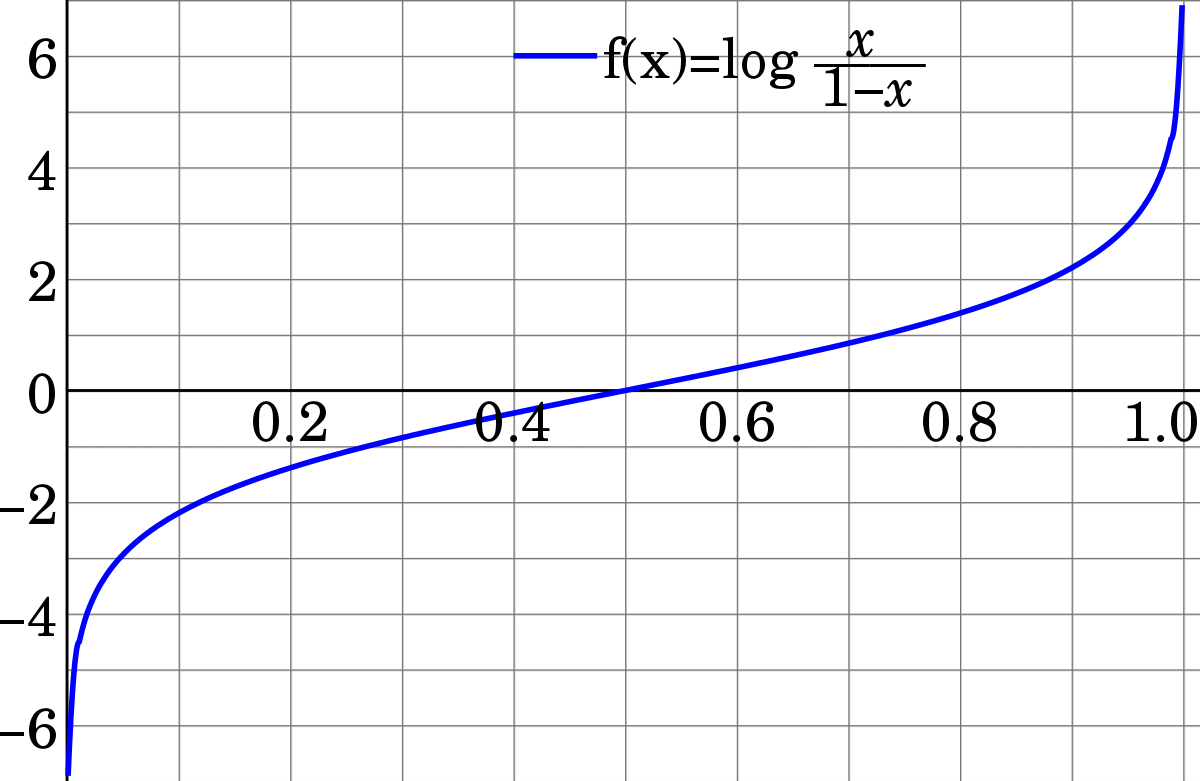
\includegraphics[width=0.5\textwidth]{logit.png}
    \caption{Logit funkcija}\label{fig:prettypic}
\end{figure}
\begin{figure}
    \centering
    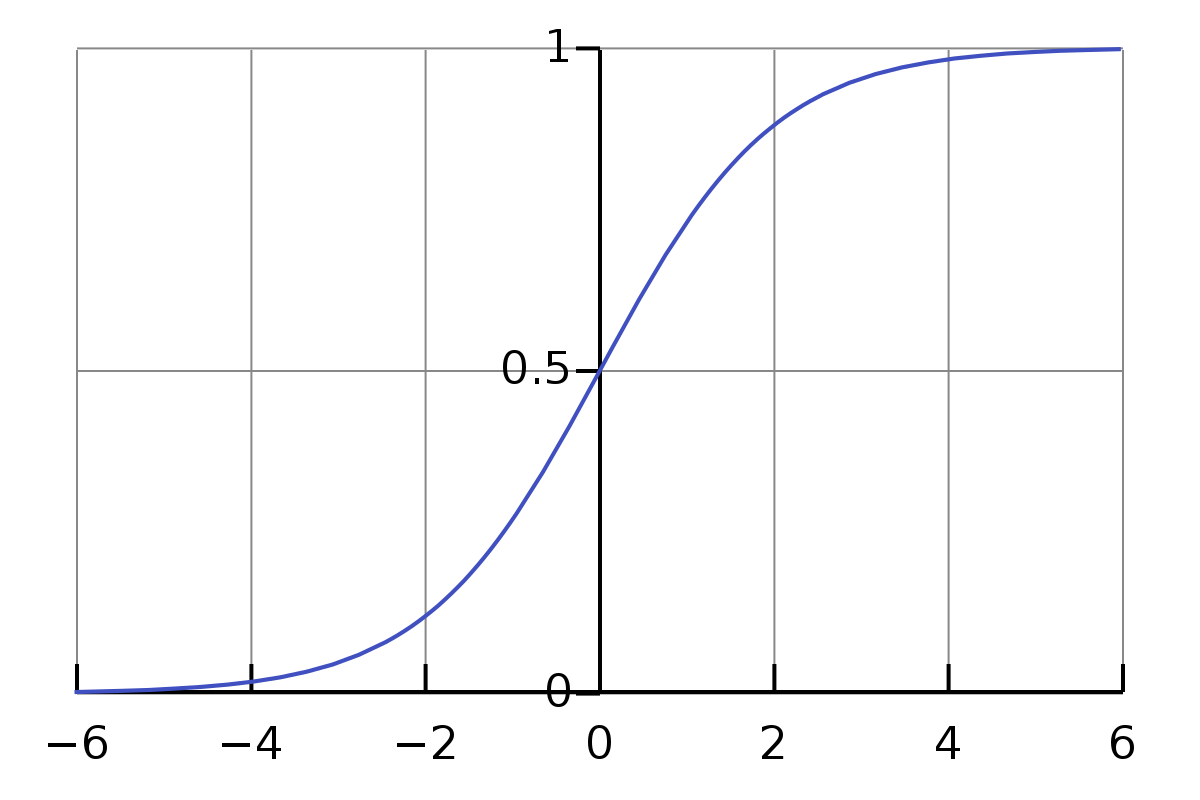
\includegraphics[width=0.5\textwidth]{logistic.png}
    \caption{Logistička funkcija}\label{fig:prettypic}
\end{figure}

Grafik logističke funkcije dat je na slici 2.2. Vidimo da je sada domen funkcije $ (-\infty, +\infty) $, a kodomen $ (0, +1) $. Ovakva funkcija se naziva \textit{sigmoidnom} funkcijom (takođe postoji naziv i \enquote{S}-kriva) i ona daje broj uvek između 0 i 1. \\
Kada logistička regresija nađe verovatnoću \textit{\^{p}} kao funkciju ulaznih parametara , ona na osnovu te verovatnoće može da da predikciju da li taj podatak pripada pozitivnoj klasi. 

\begin{equation}
  \textit{\^{y}} =
  \begin{cases}
    1, & \textit{\^{p}} > 0.5 \\
    0, & \textit{\^{p}} < 0.5
  \end{cases}
\end{equation}

\subsection{Treniranje modela i funkcija gubitka}

Cilj treniranja modela je da se podese parametri vektora  $\theta$ tako da model daje visoku verovatnoću za pozitivne instance (y = 1) i nisku verovatnoću za negativne instance (y = 0).  Funkcija gubitka se koristi kada se optimizuju parametri modela. Funkcija gubitka mapira neku realnu vrednost, najčešće je to nekakva razlika predviđene vrednosti i stvarne vrednosti labele neke instance, u realan broj. Taj realan broj predstavlja cenu. Cilj optimizacije modela je da minimizira funkciju gubitka. Početni izgled funkcije gubitka za logističku regresiju je dat u jednačini . 

\begin{equation} \label{eq:f-ja kostanja}
  \textit{c($\theta$)} =
  \begin{cases}
    -ln($\^{p}$), &  y = 1 \\
    -ln(1 - $\^{p}$), & y = 0
  \end{cases}
\end{equation}

\begin{figure}
    \centering
    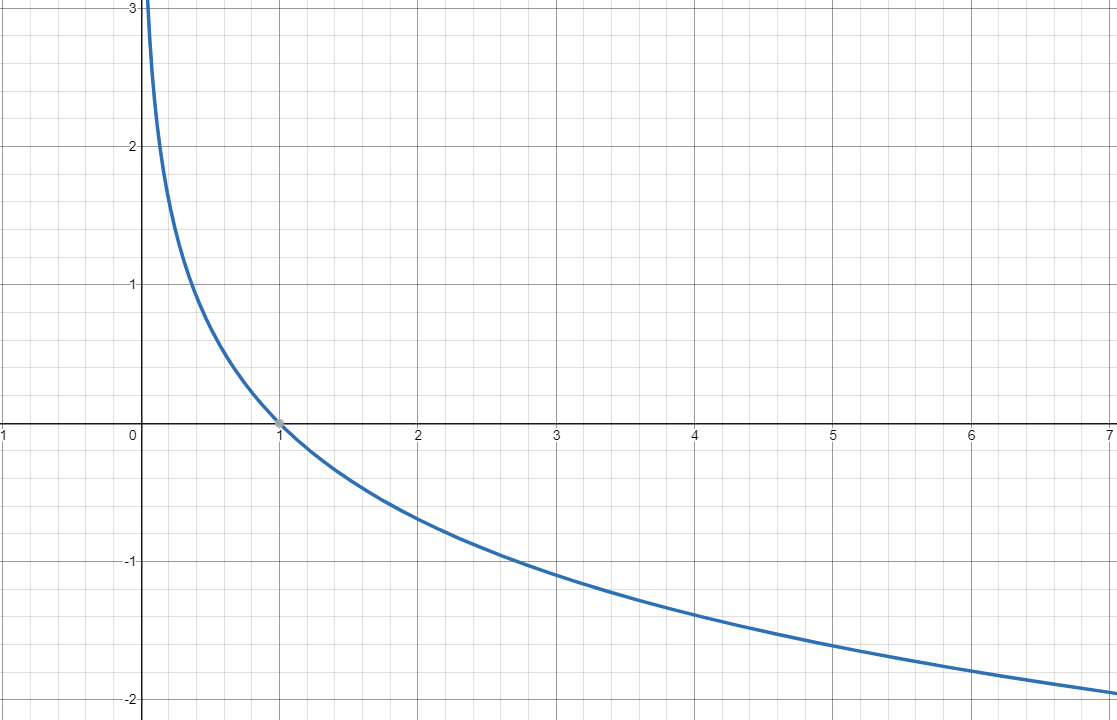
\includegraphics[width=0.5\textwidth]{neglog.png}
    \caption{Grafik funkcije -ln(x)}\label{fig:neglog}
\end{figure}

Na slici \ref{fig:neglog} je dat grafik funkcije $-ln(x)$. Kada $x \to 0$ , tada $ -ln(x) \to \infty $. Zbog toga će cena biti velika ako model proceni verovatnoću koja teži nuli za pozitivne instance. Takođe biće jako velika ako model proceni verovatnoću blizu jedinice za negativne instance. Ako je x u okolini jedinice, tada će -ln(x)  imati vrednost oko nule. Odnosno ako cena će biti 0 ako je procenjena verovatnoća blizu 0 za negativne instance, ili blizu 1 za pozitivne instance. Funkcija \ref{eq:f-ja kostanja} se može takođe napisati kao:
\begin{equation} \label{eq:logloss}
	 \textit{c($\theta$)} = [\ y ln(\hat{p}) + (1 - y)ln(1 - \hat{p}) ]\
\end{equation}
Odnosno za sve elemente ulazne matrice dobijamo konačni oblik, dat u jednačini \ref{eq:loglossfinal}. 
\begin{equation} \label{eq:loglossfinal}
	 J(\theta) = -  \frac{1}{m} \sum_{i=1}^{m} [\ y^i ln(\hat{p}^i) + (1 - y^i)ln(1 - \hat{p}^i) ]\
\end{equation}

Konstanta $\frac{1}{m}$ se koristi da bi se našla prosečna vrednost svih grešaka. Jednačina zatvorenog oblika koja optimalne izračunava vrednosti $\theta$ vektora nije poznata. Međutim ova funkcija jeste konveksna, tako da se optimizacionim algoritmom opadajućeg gradijenta može naći globalni minimum funkcije. Za globalni minimum funkcije gubitaka svi parametri vektora $\theta$ imaju optimalne vrednosti, odnosno najmanja je razlika između pravih labela i procenjenih labela. Kada se stigne do globalnog minimuma nije više moguće smanjivati razliku između procenjene i realne vrednosti. \\

U nastavku biće dat postupak dobijanja gradijenta funkcije \ref{eq:loglossfinal}. Biće dat postupak dobijanja parcijalnog izvoda po promenljivoj $\theta \textsubscript{j}$. Gradijent funkcije je specijalan slučaj Jakobijeve matrice, kada je funkcija skalarna. U opštem slučaju gradijent skalarne diferencijabilne funkcije više promenljih je vektorsko polje $ \nabla $ \textit{f} čija vrednost u tački \textit{p} je vektor čije komponente su parcijalni izvodi \textit{f} u \textit{p}. Odnosno za \textit{f}: $ \rm I\!R  ^ n \to \rm I\!R $, njen gradijent je definisan kao: $ \nabla $ \textit{f}: $ \rm I\!R  ^ n \to \rm I\!R ^ n $   je definisan u tački \textit{p} = (x\textsubscript{1}, x\textsubscript{2}, ..., x\textsubscript{n}) u n-to dimenzionalnom prostoru kao vektor:

\begin{equation}
\begin{split}
\nabla \textit{f(p)} = 
\begin{pmatrix} \frac{\partial f}{\partial x \textsubscript{1}} \\\\ \frac{\partial f}{\partial x\textsubscript{2}} \\.\\ .\\.\\ \frac{\partial f}{\partial x\textsubscript{n}} \end{pmatrix}
\end{split}
\end{equation}

Gradijent vektor se može protumačiti kao \enquote{pravac i stopa najbržeg rasta} funkcije. Ako je gradijent funkcije u tački \textit{p} nenulti, pravac gradijenta je pravac u kome funkcija najbrže raste od tačke \textit{p}. Intenzitet gradijenta je stopa rasta u tom pravcu. Gradijent je nulti vektor u tački samo ako je to stacionarna tačka, tj. ako je to tačka ekstremuma. Kasnije će biti potrebno da iterativnim metodama smanjujemo vrednost funkcije i za ovo će nam biti potreban negativan gradijent funkcije, umesto pozitivnog.\\

\textbf{Izvod logističke funkcije}\\

U nastavku je dat izvod logističke funkcije $\sigma(x)  = \frac{1}{1+e^{-x}}$.

\begin{equation}
\begin{split}
	\frac{\partial (\sigma(x))}{\partial x} & = \frac{0 * (1 + e^{-x}) - (1)*(e^{-x}*(-1))}{({1+e^{-x}})^2} \\
 		& = \frac{ e^{-x}}{({1+e^{-x}})^2} = \frac{1-1 + e^{-x}}{({1+e^{-x}})^2}= \frac{ 1 + e^{-x}}{({1+e^{-x}})^2} - \frac{1}{({1+e^{-x}})^2} \\
 		& = \frac{1}{1+e^{-x}} * \left( 1 - \frac{1}{1+e^{-x}}\right) = \sigma(x)(1-\sigma(x))
\end{split}
\end{equation}

\textbf{Izvod funkcije gubitaka}\\

U nastavku je dat izvod funkcije gubitaka \ref{eq:loglossfinal}.\\

\textbf{Korak 1: Nalaženje diferencijala složene funkcije:}

\begin{equation}
\begin{split}
	\frac{\partial (J(\theta))}{\partial \theta\textsubscript{j}} & = -  \frac{1}{m} \left( \sum_{i=1}^{m} \left[\ y^i * \frac{1}{h\textsubscript {$\theta$} (x^i)}  * \frac{\partial (h\textsubscript {$\theta$}(x^i)}{\partial \theta\textsubscript{j}}\right] + \sum_{i=1}^{m} \left[\ (1 - y^i) * \frac{1}{1 - h\textsubscript {$\theta$} (x^i)}    * \frac{\partial (1 -h\textsubscript {$\theta$}(x^i)}{\partial \theta\textsubscript{j}}\right]\ \right) \\
 		& = - \frac{1}{m} \left( \sum_{i=1}^{m} \left[\ y^i * \frac{1}{h\textsubscript {$\theta$} (x^i)} * \sigma(z)(1-\sigma(z))  * \frac{\partial (\theta^T x)}{\partial \theta\textsubscript{j}} \right] \right) \\ 
 		& - \frac{1}{m} \left( \sum_{i=1}^{m} \left[\ (1 - y^i) * \frac{1}{1 - h\textsubscript {$\theta$} (x^i)} * -\sigma(z)(1-\sigma(z))  * \frac{\partial (\theta^T x)}{\partial \theta\textsubscript{j}}\right]\ \right) \\
\end{split}
\end{equation}

\textbf{Korak 2: Zamena sigmoidne funkcije i nalaženje diferencijala argumenta:} 

\begin{equation}
\begin{split}
	\frac{\partial (J(\theta))}{\partial \theta\textsubscript{j}} & = - \frac{1}{m} \left( \sum_{i=1}^{m} \left[\ y^i * \frac{1}{h\textsubscript {$\theta$} (x^i)} * \sigma(z)(1-\sigma(z))  * \frac{\partial (\theta^T x)}{\partial \theta\textsubscript{j}} \right] \right) \\ 
 		& - \frac{1}{m} \left( \sum_{i=1}^{m} \left[\ (1 - y^i) * \frac{1}{1 - h\textsubscript {$\theta$} (x^i)} * -\sigma(z)(1-\sigma(z))  * \frac{\partial (\theta^T x)}{\partial \theta\textsubscript{j}}\right]\ \right) \\
 		& = - \frac{1}{m} \left( \sum_{i=1}^{m} \left[\ y^i * \frac{1}{h\textsubscript {$\theta$} (x^i)} * {h\textsubscript {$\theta$} (x^i)}(1-{h\textsubscript {$\theta$} (x^i)})  * x\textsubscript{j}^i \right] \right) \\ 
 		& - \frac{1}{m} \left( \sum_{i=1}^{m} \left[\ (1 - y^i) * \frac{1}{1 - h\textsubscript {$\theta$} (x^i)} * -{h\textsubscript {$\theta$} (x^i)}(1-{h\textsubscript {$\theta$} (x^i)})  * x\textsubscript{j}^i\right]\ \right) \\
\end{split}
\end{equation}
Napomena: z = \textbf{$\theta^T$x} \\

\textbf{Korak 3: Uprošćavanje množenjem:} 

\begin{equation}
\begin{split}
	\frac{\partial (J(\theta))}{\partial \theta\textsubscript{j}} & = \\
	 & = - \frac{1}{m} \left( \sum_{i=1}^{m} \left[\ y^i * (1-{h\textsubscript {$\theta$} (x^i)})  * x\textsubscript{j}^i  - (1 - y^i)  * {h\textsubscript {$\theta$} (x^i)}  * x\textsubscript{j}^i\right]\ \right) \\
	  & = - \frac{1}{m} \left( \sum_{i=1}^{m} \left[\ y^i  - y^i * {h\textsubscript {$\theta$} (x^i)} - {h\textsubscript {$\theta$} (x^i)} + y^i  * {h\textsubscript {$\theta$} (x^i)} \right]\ x\textsubscript{j}^i  \right)  \\
	   & = - \frac{1}{m} \left( \sum_{i=1}^{m} \left[\ y^i  - {h\textsubscript {$\theta$} (x^i)} \right]\ x\textsubscript{j}^i  \right)  \\
\end{split}
\end{equation}

\section{Softmaks regresija}

\chapter{Implementacija}

\section{Logistička regresija}

\section{Softmaks regresija}

\chapter{Analiza rezultata}

\chapter{Primena kod neuronskih mreža}

\end{document}